\documentclass[a4paper,12pt]{article}
\usepackage[top = 2.5cm, bottom = 2.5cm, left = 2.5cm, right = 2.5cm]{geometry}
% Unfortunately, LaTeX has a hard time interpreting German Umlaute. The following two lines and packages should help. If it doesn't work for you please let me know.
\usepackage[T1]{fontenc}
\usepackage[utf8]{inputenc}
% The following two packages - multirow and booktabs - are needed to create nice looking tables.
\usepackage{multirow} % Multirow is for tables with multiple rows within one cell.
\usepackage{booktabs} % For even nicer tables.
% As we usually want to include some plots (.pdf files) we need a package for that.
\usepackage{graphicx}
% The default setting of LaTeX is to indent new paragraphs. This is useful for articles. But not really nice for homework problem sets. The following command sets the indent to 0.
\usepackage[spanish]{babel}
\usepackage{setspace}
\setlength{\parindent}{0in}
% Package to place figures where you want them.
\usepackage{float}
% The fancyhdr package let's us create nice headers.
\usepackage{fancyhdr}
\usepackage{amsmath}
\usepackage{amssymb}
\usepackage{amsthm}
\usepackage{natbib}
\usepackage{graphicx}
\usepackage{subcaption}
\usepackage{booktabs}
\usepackage{etoolbox}
\AtBeginEnvironment{align}{\setcounter{equation}{0}}

\pagestyle{fancy}

\fancyhf{}

\lhead{\footnotesize Tarea 1}
\rhead{\footnotesize  Rompich}
\cfoot{\footnotesize \thepage}

\begin{document}
    \thispagestyle{empty} % This command disables the header on the first page.

    \begin{tabular}{p{15.5cm}} % This is a simple tabular environment to align your text nicely
    \begin{tabbing}
    Universidad del Valle de Guatemala \\ 23 de enero de 2021  \\
    Rudik R. Rompich   - Carné: 19857\\
    \end{tabbing}
    Ecuaciones Diferenciales 2 - Dorval Carías \\
    \hline % \hline produces horizontal lines.
    \\
    \end{tabular} % Our tabular environment ends here.
    \vspace*{0.3cm} % Now we want to add some vertical space in between the line and our title.
    \begin{center} % Everything within the center environment is centered.
    {\Large \bf Tarea 1
} % <---- Don't forget to put in the right number
        \vspace{2mm}
    \end{center}
    \vspace{0.4cm}

1. Sea $z \in \mathbb{C}, z \neq 0$. Encuentre las condiciones para que $z+\frac{1}{z} \in \mathbb{R}$.\newline\newline 
\begin{proof}
\textit{Demostración:}
\begin{align}
    \text{Sea } z=x+iy\\
    \implies& z+\frac{1}{z} = x+iy +\frac{1}{x+iy}\implies x+iy +\frac{1}{x+iy}\cdot \frac{x-iy}{x-iy}\\
    \implies& x+iy +\frac{x-iy}{x^2-xyi+xyi-i^2y^2}\implies x+iy +\frac{x-yi}{x^2+y^2}\\
    \implies& x+\frac{x}{x^2+y^2}+iy-\frac{yi}{x^2+y^2}\implies \frac{x(x^2+y^2)+x}{x^2+y^2}+\frac{iy(x^2+y^2)-yi}{x^2+y^2}\\
    \implies& \frac{x(x^2+y^2+1)}{x^2+y^2}+i\frac{y(x^2+y^2-1)}{x^2+y^2}\\
    \implies& z+\frac{1}{z} \in \mathbb{R}\Longleftrightarrow x^2+y^2 =1 \lor b=0.
\end{align}
\end{proof}
2. Muestre que una ecuación para el circulo $C\left(z_{0}, r\right)$ en el plano complejo es:
$z \bar{z}-z_{0} \bar{z}-z \overline{z_{0}}+z_{0} \overline{z_{0}}=r^{2}$\newline 
\begin{proof}
\begin{align}
    \implies& \bar{z}-z_{0} \bar{z}-z \overline{z_{0}}+z_{0} \overline{z_{0}}=r^{2}\\
    \implies& z(\bar{z}-\bar{z}_0)-z_0(\bar{z}-\bar{z}_0)=r^{2}\\
    \implies& (z-z_0)(\bar{z}-\bar{z}_0)=r^{2}\\
    \implies& (z-z_0)\bar{(z-z_0)}=r^{2}\\
    \implies& |z-z_0|^2=r^{2}, \text{ si } |z-z_0|=r\\
    \implies& |z-z_0|^2=r^2
\end{align}
\end{proof}
3 .
\begin{enumerate}
    \item Encuentre las raíces quintas de la unidad.
    \begin{align}
        \implies& z^5=1 \\
        \implies& r=\sqrt{(1)^2+(0)}=1 \qquad \theta=arg(Z) = \tan \theta=\frac{0}{1}=0\\
        \implies& t=1\qquad r=1\qquad arg(Z)=1\\
        \implies& z=1\cos\theta+i\sin\theta =1\cos(0)+i(1)\sin(0)\\
        \intertext{Entonces:}
        \implies& w_k =(1)^{1/5}[\cos(\frac{0+2k\pi}{5})+i\sin(\frac{0+2k\pi}{5})]\\
        k=0&; \qquad w_0= \cos(0)+i\sin(0)\\
        k=1&; \qquad w_1= \cos(\frac{2\pi}{5})+i\sin(\frac{2\pi}{5})\\
        k=2&; \qquad w_2= \cos(\frac{4\pi}{5})+i\sin(\frac{4\pi}{5})\\
        k=3&; \qquad w_3= \cos(\frac{6\pi}{5})+i\sin(\frac{6\pi}{5})\\
        k=4&; \qquad w_4= \cos(\frac{8\pi}{5})+i\sin(\frac{8\pi}{5})
    \end{align}
    \item Encuentre todas las soluciones complejas de $z^{6}=-8 i$.
    \begin{align}
        x=0\quad y=-8 \\
        \implies& r=\sqrt{0^2+(-8)^2}=8\quad arg(Z)=\theta=-\frac{\pi}{2}\\
        \implies& 8\cos(-\frac{\pi}{2})+i(8\sin(-\frac{\pi}{2}))\\
        w_k&=(8)^{1/6}\left[\cos\left(\frac{-\frac{\pi}{2}+2k\pi}{6} \right)+i\sin\left(\frac{-\frac{\pi}{2}+2k\pi}{6} \right) \right]\\
        w_0 &=(8)^{1/6}\left[\cos\left(\frac{-\frac{\pi}{2}}{6} \right)+i\sin\left(\frac{-\frac{\pi}{2}}{6} \right) \right]\\
        &=(8)^{1/6}\left[\frac{\sqrt{6}+\sqrt{2}}{4}+i\left(\frac{\sqrt{6}+\sqrt{2}}{4} \right) \right]\\
        w_1 &=(8)^{1/6}\left[\cos\left(\frac{-\frac{\pi}{2}+2\pi}{6} \right)+i\sin\left(\frac{-\frac{\pi}{2}+2\pi}{6} \right) \right]\\
        &=(8)^{1/6}\left[\frac{\sqrt{2}}{2}+i\frac{\sqrt{2}}{2}\right]\\
        w_2 &=(8)^{1/6}\left[\cos\left(\frac{-\frac{\pi}{2}+4\pi}{6} \right)+i\sin\left(\frac{-\frac{\pi}{2}+4\pi}{6} \right) \right]\\
        &=(8)^{1/6}\left[\frac{-(\sqrt{3}-1)\sqrt{2}}{4}+i\frac{(\sqrt{3}+1)\sqrt{2}}{4}\right]\\
        w_3 &=(8)^{1/6}\left[\cos\left(\frac{-\frac{\pi}{2}+6\pi}{6} \right)+i\sin\left(\frac{-\frac{\pi}{2}+6\pi}{6} \right) \right]\\
        &=(8)^{1/6}\left[\frac{-(\sqrt{3}-1)\sqrt{2}}{4}+i\frac{(\sqrt{3}+1)\sqrt{2}}{4}\right]\\
        w_4 &=(8)^{1/6}\left[\cos\left(\frac{-\frac{\pi}{2}+8\pi}{6} \right)+i\sin\left(\frac{-\frac{\pi}{2}+8\pi}{6} \right) \right]\\
        &=(8)^{1/6}\left[-\frac{\sqrt{2}}{2}-i\frac{\sqrt{2}}{2}\right]\\
        w_5 &=(8)^{1/6}\left[\cos\left(\frac{-\frac{\pi}{2}+10\pi}{6} \right)+i\sin\left(\frac{-\frac{\pi}{2}+10\pi}{6} \right) \right]\\
        &=(8)^{1/6}\left[\frac{-(\sqrt{3}-1)\sqrt{2}}{4}+i\frac{(\sqrt{3}+1)\sqrt{2}}{4}\right]
    \end{align}
\end{enumerate}

4. Compruebe las identidades trigonométricas a continuación:
\begin{enumerate}
    \item $\cos 5 \theta=16 \cos ^{5} \theta-20 \cos ^{3} \theta+5 \cos \theta$
    \begin{align}
        \cos 5\theta &= \cos(3\theta+2\theta) \\
        &= \cos3\theta\cos2\theta-\sin3\theta\sin2\theta \\
        &= (4\cos^3\theta -3\cos\theta)(2\cos^2\theta -1)-(3\sin\theta-4\sin^3\theta)(2\sin\theta\cos\theta)\\
        &=\left(8 \cos ^{5} \theta-10 \cos ^{3} \theta+3 \cos \theta\right)-\left(3-4 \sin ^{2} \theta\right)\left(2 \sin ^{2} \theta \cos \theta\right)\\
&=\left(8 \cos ^{5} \theta-10 \cos ^{3} \theta+3 \cos \theta\right)-\left(3-4\left(1-\cos ^{2} \theta\right)\right)\left(2\left(1-\cos ^{2} \theta\right) \cos \theta\right)\\
&=\left(8 \cos ^{5} \theta-10 \cos ^{3} \theta+3 \cos \theta\right)-\left(3-4+4 \cos ^{2} \theta\right) \left(2 \cos \theta-2 \cos ^{3} \theta\right)\\
&=\left(8 \cos ^{5} \theta-10 \cos ^{3} \theta+3 \cos \theta\right)-\left(-8 \cos ^{5} \theta+10 \cos ^{3} \theta-2 \cos \theta\right)\\
&= 16 \cos ^{5} \theta-20 \cos ^{3} \theta+5 \cos \theta
    \end{align}
    
    \item $(\operatorname{sen} 5 \theta) /(\operatorname{sen} \theta)=16 \cos ^{4} \theta-12 \cos ^{2} \theta+1, \theta \neq 0, \pm \pi, \pm 2 \pi, \cdots$
    \begin{align}
    \intertext{Primero se determina $\sin5\theta$}
\sin 5 \theta &=\sin (3 \theta+2 \theta) \\
&=\sin 3 \theta \cos 2 \theta+\cos 3 \theta \sin 2 \theta \\
&=\left(3 \sin \theta-4 \sin ^{3} \theta\right)\left(1-\sin^{2} \theta\right)+\left(4 \cos ^{3} \theta-3 \cos \theta\right)(2 \sin \theta \cos \theta) \\
&=\sin \theta\left[\left(3-4 \sin ^{2} \theta\right)\left(2 \cos ^{2} \theta-1\right)+\left(4 \cos ^{3} \theta-3 \cos \theta\right)(\cos \theta)\right]
\intertext{Entonces:}
\frac{\sin 5 \theta}{\sin \theta} &=\left[\left(3-4\left(1-\cos ^{2} \theta\right)\right]\left(2 \cos ^{2} \theta-1\right)+\left(8 \cos ^{4} \theta-6 \cos ^{2} \theta\right)\right] \\
&=\left[\left(3-4+4 \cos ^{2} \theta\right)\left(2 \cos ^{2} \theta-1\right)+8 \cos ^{4} \theta-6 \cos ^{2} \theta\right) \\
&=\left[\left(-1+4 \cos ^{2} \theta\right)\left(2 \cos ^{2} \theta-1\right)+3\cos ^{4} \theta-6 \cos ^{2} \theta\right) \\
&=\left(-2 \cos ^{2} \theta+8 \cos ^{4} \theta+1-4 \cos ^{2} \theta+8 \cos ^{4} \theta-6 \cos ^{2} \theta\right)\\
&= 16 \cos ^{4} \theta-12 \cos ^{2} \theta+1, \theta \neq 0, \pm \pi, \pm 2 \pi, \cdots
\end{align}
\end{enumerate}
5. Realice las operaciones indicadas:

\begin{enumerate}
    \item $(-1+i)^{1 / 3}$
    \begin{align}
        \intertext{Se puede representar como: $z^3= (-1+i)$}
        \intertext{Entonces $x=-1$ y $y=1$. Por lo que $argZ=-\frac{\pi}{4}$ y $r=\sqrt{2}$}
        \implies& w_k =(\sqrt{2})^{1/3}[\cos(\frac{-\frac{\pi}{4}+2k\pi}{3})+i\sin(\frac{-\frac{\pi}{4}+2k\pi}{3})]\\
        \implies& w_0 =(\sqrt{2})^{1/3}[\cos(\frac{-\frac{\pi}{4}}{3})+i\sin(\frac{-\frac{\pi}{4}}{3})]\\
        \implies& w_1 =(\sqrt{2})^{1/3}[\cos(\frac{-\frac{\pi}{4}+2\pi}{3})+i\sin(\frac{-\frac{\pi}{4}+2\pi}{3})]\\
        \implies& w_2 =(\sqrt{2})^{1/3}[\cos(\frac{-\frac{\pi}{4}+4\pi}{3})+i\sin(\frac{-\frac{\pi}{4}+4\pi}{3})]
    \end{align}
    \item  $(-2 \sqrt{3}-2 i)^{1 / 4}$
    \begin{align}
        \intertext{Se puede representar como: $z^4= (-2\sqrt{3}-2i)$}
        \intertext{Entonces $x=-2\sqrt{3}$ y $y=-2$. Por lo que $argZ=\frac{\pi}{6}$ y $r=4$}
         \implies& w_k =(\sqrt{4})^{1/4}[\cos(\frac{\frac{\pi}{6}+2k\pi}{4})+i\sin(\frac{-\frac{\pi}{5}+2k\pi}{4})]\\
         \implies& w_0 =(\sqrt{4})^{1/4}[\cos(\frac{\frac{\pi}{6}}{4})+i\sin(\frac{-\frac{\pi}{5}}{4})]\\
         \implies& w_1
         =(\sqrt{4})^{1/4}[\cos(\frac{\frac{\pi}{6}+2\pi}{4})+i\sin(\frac{-\frac{\pi}{5}+2\pi}{4})]\\
         \implies& w_2
         =(\sqrt{4})^{1/4}[\cos(\frac{\frac{\pi}{6}+4\pi}{4})+i\sin(\frac{-\frac{\pi}{5}+4\pi}{4})]\\
         \implies& w_3 =(\sqrt{4})^{1/4}[\cos(\frac{\frac{\pi}{6}+6\pi}{4})+i\sin(\frac{-\frac{\pi}{5}+6\pi}{4})]
    \end{align}
    \item  $\sqrt{-15-8 i}$
    \begin{align}
        \intertext{Se puede representar como: $z^2= (-15-8i)$}
        \intertext{Entonces $x=-15\sqrt{3}$ y $y=-8$. Por lo que $argZ=0.3$ y $r=17$}
         \implies& w_k =(\sqrt{17})^{1/2}[\cos(\frac{0,3+2k\pi}{2})+i\sin(\frac{0,3+2k\pi}{2})]\\
         \implies& w_0 =(\sqrt{17})^{1/2}[\cos(\frac{0,3}{2})+i\sin(\frac{0,3}{2})]\\
         \implies& w_1 =(\sqrt{17})^{1/2}[\cos(\frac{0,3+2\pi}{2})+i\sin(\frac{0,3+2\pi}{2})]\\
    \end{align}
\end{enumerate}
6. Resuelva las ecuaciones siguientes:
\begin{enumerate}
    \item $z^{2}+(2 i-3) z+5-i=0$
    \begin{align}
    \intertext{Supóngase $a=1,b=(2i-3),c=5-i$}
    \implies z&= \frac{-(2i-3)\pm\sqrt{(2i-3)^2-4(5-i)}}{2}\\
    &= \frac{(-2i-3)\pm\sqrt{-12i+5-20+4i}}{2}\\
    &= \frac{3-2i\pm i\sqrt{8i+15}}{2}
    \intertext{En donde $\sqrt{8i+15}=16+8i-1=16+8i+i^2=(i+4)^2$}
    &= \frac{3-2i\pm i(i+4)}{2}
    \intertext{Entonces:}
    z_1&= \frac{2+2i}{2}=1+i\\
    z_2&= \frac{4-2i}{2}=2-i
    \end{align}
    \item $6 z^{4}-25 z^{3}+32 z^{2}+3 z-10=0$
    \begin{align}
        \intertext{Luego de una larga factorización por división sintética...}
        6 z^{4}-25 z^{3}+32 z^{2}+3 z-10=(2z+1)(3z-2)(z^2-4z+5)
        \intertext{Se obtiene: $z_1=-\frac{1}{2}$ y $z_2=\frac{2}{3}$}
        z_3=\frac{-(-4)\pm \sqrt{(-4)^2-4(1)(5)}}{2}=\\
        = \frac{4\pm \sqrt{-4}}{2}=\frac{4\pm 2i}{2}=\\
        = 2\pm i
    \end{align}
    \item $z^{2}\left(1-z^{2}\right)=16$
    \begin{align}
        z^2-z^4-16=0\\
        -z^4+z^2-16=0\\
        -z^4+z^2-16=0\\
        z^4-z^2+16=0\\
    \intertext{Si asumimos que $z^2=x$}
    x^2-x+16=0\\
    \intertext{Aplicando la fórmula cuadrática:}
    x= \frac{-(-1)\pm \sqrt{(-1)^2-4(1)(16)}}{2}= \frac{1\pm \sqrt{1-64}}{2}\\
    =\frac{1\pm \sqrt{-63}}{2}=\frac{1\pm\sqrt{63}i}{2}\\
    \implies x= \frac{1\pm\sqrt{63}i}{2}\implies z^2= \frac{1\pm\sqrt{63}i}{2}\\
    z= \pm \sqrt{\frac{1\pm3\sqrt{7}i}{2}}
    \end{align}
\end{enumerate}

7. Represente gráficamente el conjunto de valores de $z$ para los cuales:
\begin{enumerate}
    \item $\left|\frac{z-3}{z+3}\right|=2$
    \begin{align}
        \intertext{$z=x+iy\implies \left|\frac{x+iy-3}{x-iy+3}\right|=2$}
        &\implies |x+iy-3|=2|x+iy+3|\\
        &\implies (x-3)^2+y^2= 4[(x+3)^2+y^2]
    \end{align}
    \begin{center}
        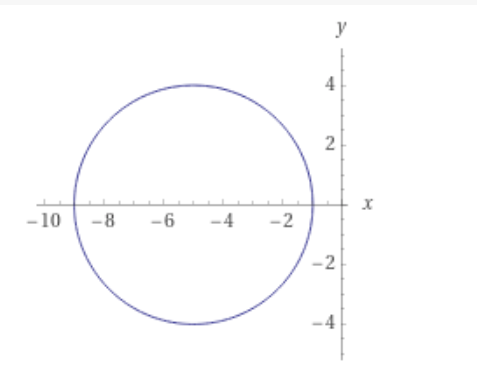
\includegraphics[scale=0.5]{1.png}
    \end{center}
   
    
    \item $\left|\frac{z-3}{z+3}\right|<2$\newline 
    \begin{center}
        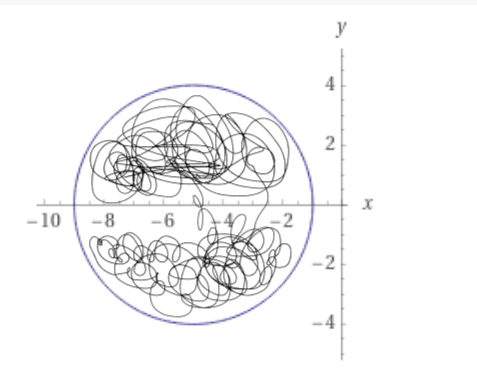
\includegraphics[scale=0.5]{2.png}
    \end{center}
    
    
\end{enumerate}
8. Un número algebraico es un número que es solución de una ecuación polinómica de la forma:
$$
a_{n} z^{n}+a_{n-1} z^{n-1}+\cdots a_{1} z+a_{0}=0
$$
donde $a_{0}, a_{1}, \cdots, a_{n}$ son enteros. Compruebe que los números siguientes son algebraicos.
\begin{enumerate}
    \item $\sqrt{3}+\sqrt{2}$
    \begin{align}
        \intertext{Supóngase $x=\sqrt{3}+\sqrt{2}$}
        \implies& (\sqrt{3}+\sqrt{2})^2=2+\sqrt{3}\sqrt{2}+2\\
        \implies& x^2=5+2\sqrt{6}\\ \implies& (x^2-5)^2=(2\sqrt{6})^2\\
        \implies& (x^2-5)^2=24
    \end{align}
    \item $\sqrt[3]{4}-2 i$
    \begin{align}
        \intertext{Supóngase $x=\sqrt[3]{4}+2i$}
        \implies x^2=(\sqrt[3]{4}+2i)^2\\
        \implies x^2= (4^{2/3}+4\sqrt[3]{4}i+4i^2)\\
        \implies x^2= (4^{2/3}-4+4\sqrt[3]{4})\\
        \implies (x^2+4-4^{2/3})^2=16\cdot 4^{2/3}i
    \end{align}
\end{enumerate}



\end{document}